\documentclass{article}
\usepackage{cmap}
\usepackage[utf8]{inputenc}
\usepackage[english,ukrainian]{babel}
\usepackage{graphicx}
\usepackage{geometry}
\usepackage{listings}
\usepackage{amsmath}
\geometry{
	a4paper,
	left=20mm,
	right=20mm,
	top=20mm,
	bottom=20mm
}
\lstset{
	language=c,
	tabsize=4,
	keepspaces,
	showstringspaces=false,
}
\graphicspath{ {./pictures} }
\setlength{\parindent}{4em}

\newcommand\subject{Операційні системи}
\newcommand\lecturer{старший викладач кафедри ПЗ\\Грицай О.Д.}
\newcommand\teacher{старший викладач кафедри ПЗ\\Грицай О.Д.}
\newcommand\mygroup{ПЗ-22}
\newcommand\lab{2}
\newcommand\theme{Ознайомлення та керування процесами в операційних системах для
	персонального комп’ютера. Linux та MacOS}
\newcommand\purpose{Ознайомитися з процесами та потоками в операційних системах
	Linux, MacOS. Навчитися працювати із системними утилітами, що дають
	можливість отримувати інформацію про процеси, потоки, використовувану
	ними пам'ять, та іншу необхідну інформацію}

\begin{document}
\begin{normalsize}
	\begin{titlepage}
		\thispagestyle{empty}
		\begin{center}
			\textbf{МІНІСТЕРСТВО ОСВІТИ І НАУКИ УКРАЇНИ\\
				НАЦІОНАЛЬНИЙ УНІВЕРСИТЕТ "ЛЬВІВСЬКА ПОЛІТЕХНІКА"}
		\end{center}
		\begin{flushright}
			Інститут \textbf{КНІТ}\\
			Кафедра \textbf{ПЗ}
		\end{flushright}
		\vspace{200pt}
		\begin{center}
			\textbf{ЗВІТ}\\
			\vspace{10pt}
			До лабораторної роботи № \lab\\
			\textbf{На тему}: “\textit{\theme}”\\
			\textbf{З дисципліни}: “\subject”
		\end{center}
		\vspace{112pt}
		\begin{flushright}
			
			\textbf{Лектор}:\\
			\lecturer\\
			\vspace{28pt}
			\textbf{Виконав}:\\
			
			студент групи \mygroup\\
			Коваленко Д.М.\\
			\vspace{28pt}
			\textbf{Прийняла}:\\
			
			\teacher\\
			
			\vspace{28pt}
			«\rule{1cm}{0.15mm}» \rule{1.5cm}{0.15mm} 2022 р.\\
			$\sum$ = \rule{1cm}{0.15mm}……………\\
			
		\end{flushright}
		\vspace{\fill}
		\begin{center}
			\textbf{Львів — 2022}
		\end{center}
	\end{titlepage}
		
	\begin{description}
		\item[Тема.] \theme.
		\item[Мета.] \purpose.
	\end{description}

	\section*{Лабораторне завдання}
	\begin{enumerate}
		\item Встановити операційні системи Linux та MacOS
		\item За допомого консольних засобів ОС Linux отримати повну інформацію
		про процеси
		\item За допомогою утиліт top, htop, qps, System Monitor отримати повну
		інформацію про процеси в ОС Linux та MacOS
		\item Використовуючи консольні засоби ОС Linux та утиліти змінити
		пріоритет виконання процесу
		\item Використовуючи консольні засоби ОС Linux та сторонні утиліти
		змінити стан виконання процесу, завершити виконання заданого процесу
		\item Скомпілювати файл main.cpp представлений у лабораторній роботі №1
		(на MacOS і Linux можна командою: g++ main.cpp -pthread) і запустити
		виконуваний файл на різній кількості активних процесорів (ядер). Знайти для
		даної програми величини $A$, $S$, $p$  при різних вхідних значеннях величини $n$.
		Порівняти результати для різних операційних систем
		\item Результати лабораторної роботи оформити у звіт, у висновку надати
		порівняння моніторингу процесів у різних системах різними утилітами,
		відповідно до індивідуального варіанту
	\end{enumerate}

	\section*{Хід роботи}	
	\begin{center}
		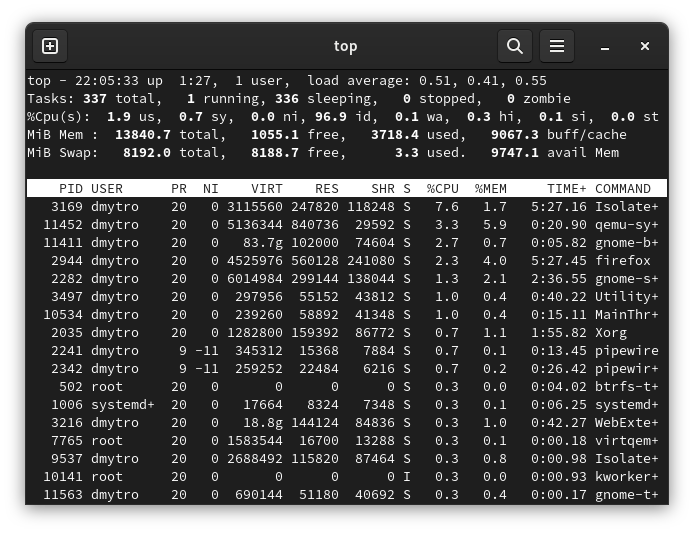
\includegraphics[scale=0.5]{top1}
	\end{center}
	\begin{center}
		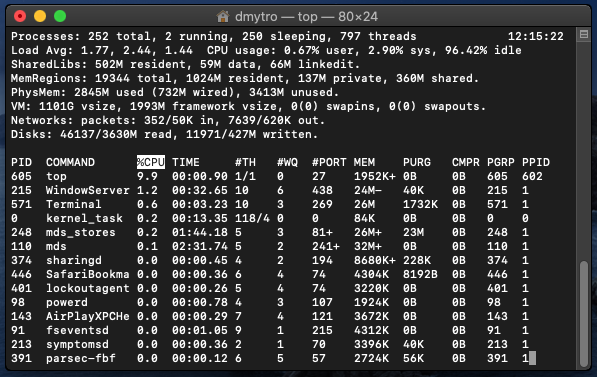
\includegraphics[scale=0.5]{top2}
	\end{center}
	\begin{center}
		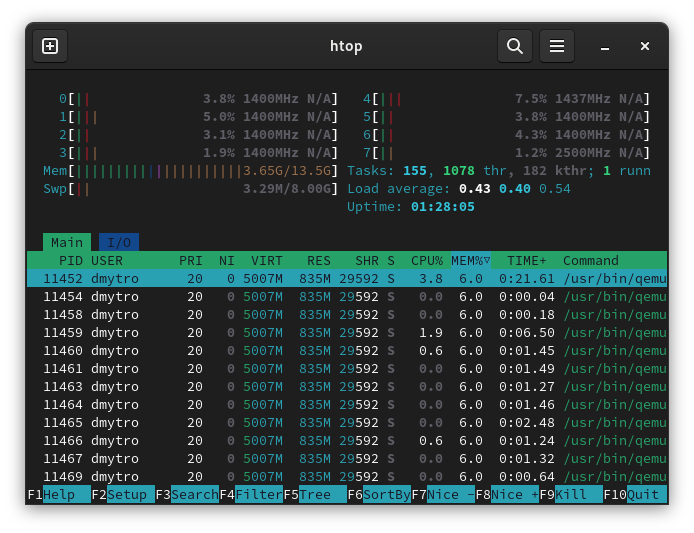
\includegraphics[scale=0.5]{htop1}
	\end{center}
	\begin{center}
		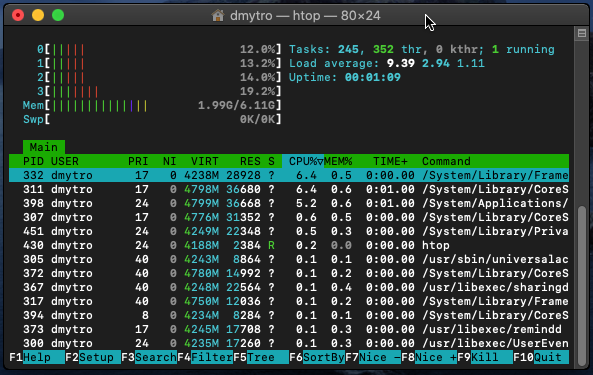
\includegraphics[scale=0.5]{htop2}
	\end{center}
	\begin{center}
		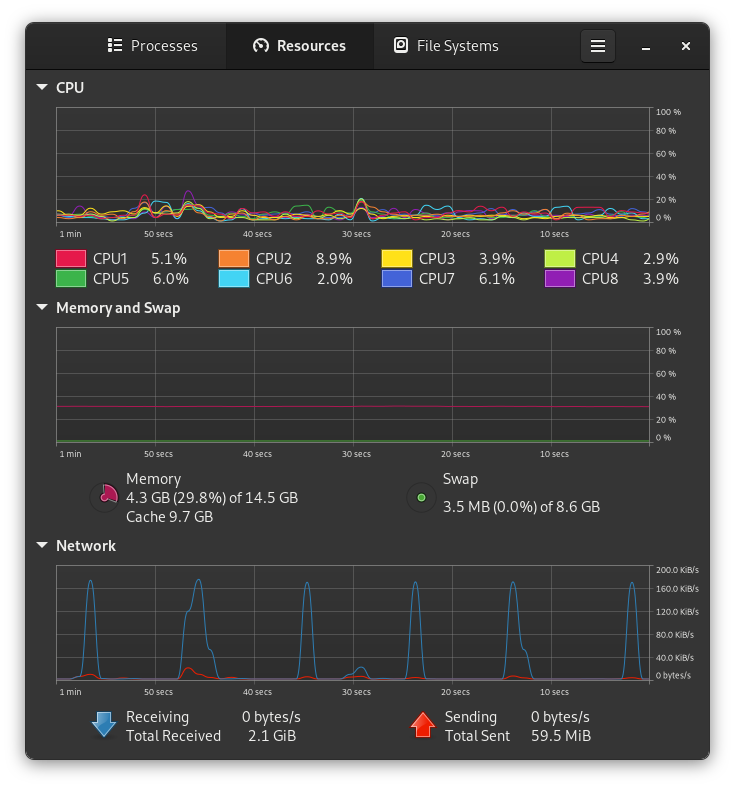
\includegraphics[scale=0.5]{sm1}
	\end{center}
	\begin{center}
		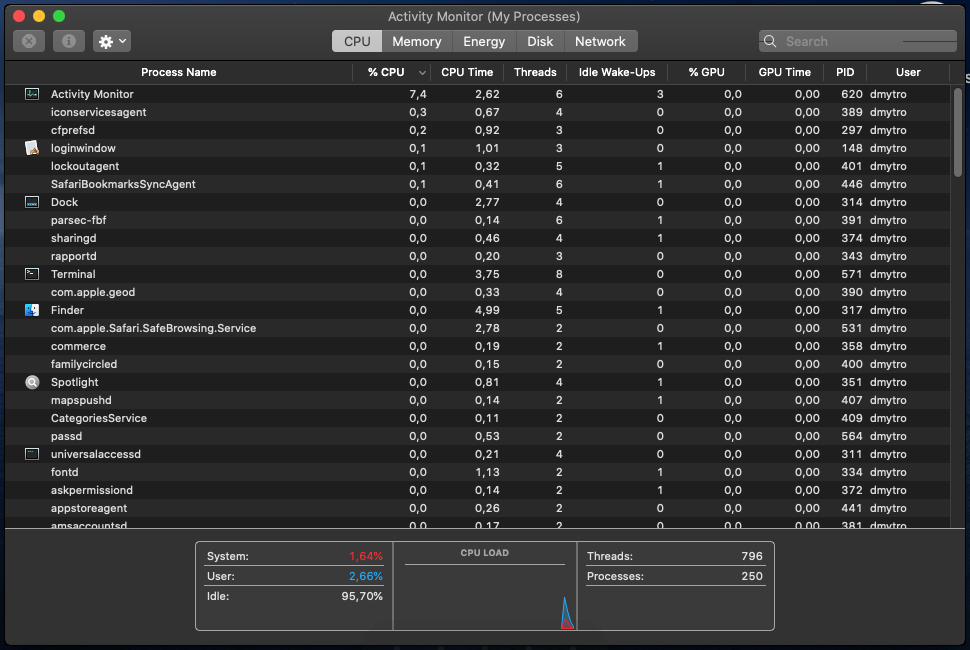
\includegraphics[scale=0.5]{sm2}
	\end{center}
	\begin{center}
		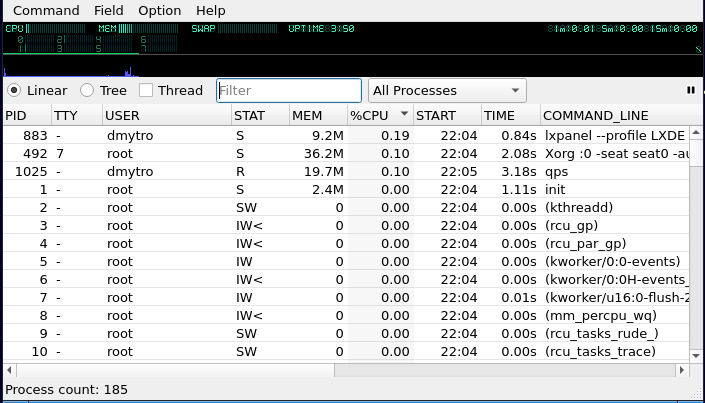
\includegraphics[scale=0.5]{qps1}
	\end{center}

	\begin{gather}
		Linux:\nonumber\\
		n=1; T_1=263\text{мс}; A=S=1; p=p.\nonumber\\
		n=2; T_2 =256\text{мс}; A=S=1.02; p=0.98.\nonumber\\
		n=3; T_3 =266\text{мс}; A=S=0.98; p=1.03.\nonumber\\
		n=4; T_4 =264\text{мс}; A=S=0.99; p=1.01.\nonumber\\
		n=5; T_5 =268\text{мс}; A=S=0.98; p=1.02.\nonumber\\
		n=6; T_6 =269\text{мс}; A=S=97; p=1.03.\nonumber\\
		n=7; T_7 =265\text{мс}; A=S=0.99; p=1.01.\nonumber\\
		n=8; T_8 =276\text{мс}; A=S=0.95; p=1.06.\nonumber\\
		MacOS:\nonumber\\
		n=1; T_1=431\text{мс}; A=S=1; p=p.\nonumber\\
		n=2; T_2 =419\text{мс}; A=S=1.02; p=0.96.\nonumber\\
		n=3; T_3 =394\text{мс}; A=S=1.09; p=0.87.\nonumber\\
		n=4; T_4 =400\text{мс}; A=S=1.07; p=0.91.\nonumber\\
		n=5; T_5 =381\text{мс}; A=S=1.13; p=0.85.\nonumber\\
		n=6; T_6 =453\text{мс}; A=S=0.95; p=1.06.\nonumber\\
		n=7; T_7 =379\text{мс}; A=S=1.13; p=0.86.\nonumber\\
		n=8; T_8 =403\text{мс}; A=S=1.06; p=0.93.\nonumber
	\end{gather}
	
	\section*{Висновок}
	Під час виконання лабораторної роботи я ознайомився з процесами та потоками в операційних системах  Linux, MacOS. Навчився працювати із системними утилітами top, htop, System Monitor та qps, що дають можливість отримувати інформацію про процеси, потоки, використовувану ними пам'ять, та іншу необхідну інформацію. 
	
	Я скомпілював представлений файл і запустив його на різній кількості активних процесорів, та знайшов для даної програми час виконання, та визначив можливе прискорення відносно початкового часу роботи.
	
	В результаті виконання лабораторної роботи я дізнався про консольні варіанти програм для моніторингу навантаження на систему та доступності ресурсів.    
\end{normalsize}
\end{document}
